\documentclass{beamer}
\usetheme{default}
\usecolortheme{dove}
\usepackage{amsmath,amssymb}
\usepackage{tikz}
\usetikzlibrary{arrows.meta,positioning,calc}

\setbeamertemplate{navigation symbols}{}
\setbeamertemplate{footline}[frame number]

\title{Gradient Flow in Joint MAP\\of Hierarchical Models}
\author{}
\date{}

\begin{document}

\begin{frame}
\titlepage
\end{frame}

%% SLIDE 1: The hierarchical model
\begin{frame}{The Hierarchical Model}

\begin{center}
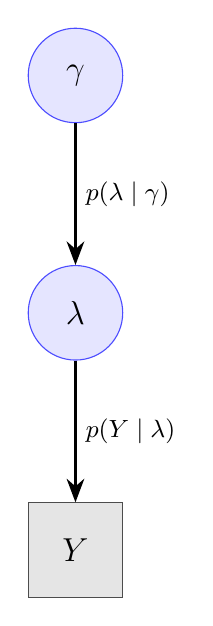
\begin{tikzpicture}[
    node distance=1.8cm,
    param/.style={circle, draw=blue!70, fill=blue!10, minimum size=1.2cm, font=\large},
    data/.style={rectangle, draw=black!70, fill=gray!20, minimum size=1.2cm, font=\large},
    arr/.style={-{Stealth[length=3mm]}, thick}
]
    \node[param] (gamma) {$\gamma$};
    \node[param, below=of gamma] (lambda) {$\lambda$};
    \node[data, below=of lambda] (Y) {$Y$};

    \draw[arr] (gamma) -- node[right, font=\small] {$p(\lambda \mid \gamma)$} (lambda);
    \draw[arr] (lambda) -- node[right, font=\small] {$p(Y \mid \lambda)$} (Y);
\end{tikzpicture}
\end{center}

\vspace{0.5cm}

\textbf{ALADYN:}
\begin{itemize}
    \item $\gamma$ = genetic effects on signatures (hyperparameter)
    \item $\lambda$ = individual latent trajectories (latent variable)
    \item $Y$ = observed disease diagnoses (data)
\end{itemize}

\end{frame}

%% SLIDE 2: Joint MAP objective
\begin{frame}{Joint MAP Objective}

Optimize \textbf{all parameters simultaneously}:

\[
\underset{\lambda,\, \gamma}{\text{argmin}} \;\; \underbrace{-\log p(Y \mid \lambda)}_{\text{NLL}} \;+\; \underbrace{-\log p(\lambda \mid \gamma)}_{\text{GP prior}}
\]

\pause
\vspace{0.5cm}

Take gradients:

\[
\frac{\partial \mathcal{L}}{\partial \lambda} = \underbrace{\frac{\partial}{\partial \lambda}\big[-\log p(Y \mid \lambda)\big]}_{\text{\color{green!60!black} data signal}} + \underbrace{\frac{\partial}{\partial \lambda}\big[-\log p(\lambda \mid \gamma)\big]}_{\text{\color{blue} prior signal}}
\]

\[
\frac{\partial \mathcal{L}}{\partial \gamma} = \underbrace{\cancel{\frac{\partial}{\partial \gamma}\big[-\log p(Y \mid \lambda)\big]}}_{\text{\color{red} zero --- $\gamma$ not in likelihood}} + \underbrace{\frac{\partial}{\partial \gamma}\big[-\log p(\lambda \mid \gamma)\big]}_{\text{\color{blue} prior signal only}}
\]

\end{frame}

%% SLIDE 3: The decoupling picture
\begin{frame}{$\lambda$ Screens $\gamma$ from the Data}

\begin{center}
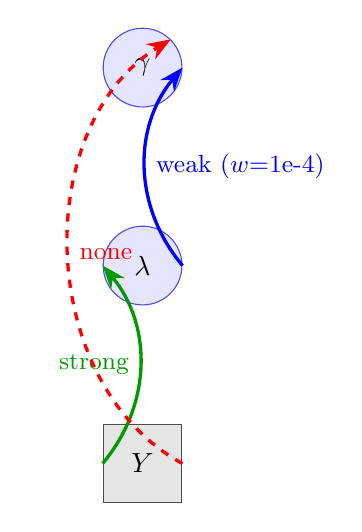
\begin{tikzpicture}[
    node distance=1.5cm,
    param/.style={circle, draw=blue!70, fill=blue!10, minimum size=1cm, font=\normalsize},
    data/.style={rectangle, draw=black!70, fill=gray!20, minimum size=1cm, font=\normalsize},
    grad/.style={-{Stealth[length=3mm]}, very thick},
]
    \node[param] (gamma) {$\gamma$};
    \node[param, below=of gamma] (lambda) {$\lambda$};
    \node[data, below=of lambda] (Y) {$Y$};

    % Gradient arrows (going UP from loss)
    \draw[grad, green!60!black] (Y.west) to[bend right=40] node[left, font=\small, text=green!60!black] {strong} (lambda.west);
    \draw[grad, blue] (lambda.east) to[bend left=40] node[right, font=\small, text=blue] {weak ($w$=1e-4)} (gamma.east);
    \draw[grad, red, dashed] (Y.east) to[bend left=60] node[right, font=\small, text=red] {none} (gamma.north east);
\end{tikzpicture}
\end{center}

\vspace{0.3cm}

\begin{itemize}
    \item $\lambda$ gets \textcolor{green!60!black}{\textbf{strong}} gradient from data
    \item $\gamma$ gets \textcolor{blue}{\textbf{weak}} gradient from prior only
    \item $\gamma$ gets \textcolor{red}{\textbf{no}} direct gradient from data
    \item[]
    \item \textbf{This is true in all joint MAP hierarchical models}
\end{itemize}

\end{frame}

%% SLIDE 4: Why it usually doesn't matter
\begin{frame}{Why It Usually Doesn't Matter}

$\lambda$ \textbf{compensates.}

\vspace{0.5cm}

\begin{columns}
\column{0.5\textwidth}
\textbf{For prediction:}
\begin{itemize}
    \item Fix $\phi, \gamma, \psi, \kappa$ from training
    \item Re-estimate $\lambda_{\text{new}}$ for each new individual
    \item $\lambda_{\text{new}}$ has $K \times T$ free parameters
    \item Adapts to new data regardless of $\gamma$ quality
\end{itemize}

\column{0.5\textwidth}
\textbf{Other examples:}
\begin{itemize}
    \item \texttt{lme4}: variance components weakly estimated, BLUPs still good
    \item Stan \texttt{optimizing}: hyperparameters only get prior gradient
    \item GAMs (\texttt{mgcv}): smoothing penalties co-estimated
\end{itemize}
\end{columns}

\vspace{0.5cm}
\pause
\textbf{It only matters when $\gamma$ is a primary scientific output.}

\end{frame}

%% SLIDE 5: The reparameterization
\begin{frame}{Reparameterization: $\lambda = \mu(\gamma) + \delta$}

\textbf{Change of variables} (same MAP, different computation graph):

\[
\underset{\delta,\, \gamma}{\text{argmin}} \;\; \underbrace{-\log p\big(Y \mid \mu(\gamma) + \delta\big)}_{\text{NLL --- $\gamma$ is inside}} \;+\; \underbrace{-\log p(\delta)}_{\text{GP prior on residual}}
\]

\pause
\vspace{0.3cm}

\begin{center}
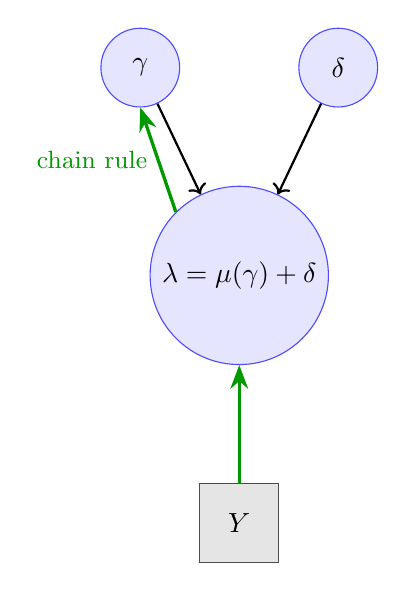
\begin{tikzpicture}[
    node distance=1.5cm,
    param/.style={circle, draw=blue!70, fill=blue!10, minimum size=1cm, font=\normalsize},
    data/.style={rectangle, draw=black!70, fill=gray!20, minimum size=1cm, font=\normalsize},
    grad/.style={-{Stealth[length=3mm]}, very thick},
]
    \node[param] (gamma) {$\gamma$};
    \node[param, right=1.5cm of gamma] (delta) {$\delta$};
    \node[param, below=1.5cm of $(gamma)!0.5!(delta)$] (lambda) {$\lambda = \mu(\gamma) + \delta$};
    \node[data, below=of lambda] (Y) {$Y$};

    \draw[thick, ->] (gamma) -- (lambda);
    \draw[thick, ->] (delta) -- (lambda);
    \draw[grad, green!60!black] (Y) -- (lambda);
    \draw[grad, green!60!black] (lambda.north west) -- node[left, font=\small, text=green!60!black] {chain rule} (gamma.south);
\end{tikzpicture}
\end{center}

\vspace{0.2cm}
Now: $\;\dfrac{\partial \mathcal{L}}{\partial \gamma} = \dfrac{\partial(-\text{NLL})}{\partial \lambda} \cdot \dfrac{\partial \mu(\gamma)}{\partial \gamma} \neq 0$ \quad {\color{green!60!black}\textbf{--- data signal!}}

\end{frame}

%% SLIDE 6: Same loss, different gradients
\begin{frame}{Same Loss, Different Gradients}

\textbf{Algebraically identical} (substitute $\delta = \lambda - \mu(\gamma)$):

\vspace{0.3cm}

\begin{tabular}{l|c|c}
 & \textbf{Original} & \textbf{Reparam} \\ \hline
Free params & $\lambda, \gamma$ & $\delta, \gamma$ \\
NLL & $-\log p(Y \mid \lambda)$ & $-\log p(Y \mid \mu(\gamma) + \delta)$ \\
Prior & $(\lambda - \mu(\gamma))^\top \Omega^{-1} (\lambda - \mu(\gamma))$ & $\delta^\top \Omega^{-1} \delta$ \\
$\gamma$ gets NLL gradient? & \color{red}{No} & \color{green!60!black}{Yes} \\
\end{tabular}

\vspace{0.5cm}
\pause

\textbf{Same stationary points.} Different optimization paths.

\vspace{0.3cm}

Analogy: minimize $f(x)$ with penalty $(x-5)^2$
\begin{itemize}
    \item Original: optimize $x$ directly
    \item Reparam: let $x = 5 + z$, optimize $z$ with penalty $z^2$
    \item Same answer --- but $5$ gets gradient from $f$ in the second form
\end{itemize}

\end{frame}

%% SLIDE 7: Empirical evidence
\begin{frame}{Empirical Evidence: ALADYN}

\begin{center}
\begin{tabular}{l|c|c}
 & \textbf{Original} & \textbf{Reparam} \\ \hline
Mean $|\gamma|$ & 0.006 & 0.081 \\
$\gamma$ correlation & \multicolumn{2}{c}{0.37} \\
$\psi$ correlation & \multicolumn{2}{c}{0.76} \\
$\phi$ correlation & \multicolumn{2}{c}{0.94} \\
\end{tabular}
\end{center}

\vspace{0.5cm}

\begin{itemize}
    \item $\phi$ (disease trajectories): nearly identical --- both fit the data well
    \item $\psi$ (disease--signature assignments): moderately different --- reparam less stable
    \item $\gamma$ (genetic effects): very different --- original $\gamma \approx 0$
    \item[]
    \item \textbf{Original $\gamma$ is effectively zero} --- genetic effects not estimated
    \item \textbf{Reparam $\gamma$ is 14$\times$ larger} --- but is it signal or overfitting?
\end{itemize}

\end{frame}

%% SLIDE 8: Summary
\begin{frame}{Summary}

\begin{enumerate}
    \item In \textbf{all} joint MAP hierarchical models, hyperparameters ($\gamma$) get no gradient from the likelihood --- only from the prior

    \vspace{0.3cm}

    \item This is \textbf{fine for prediction}: $\lambda$ compensates, and we re-estimate $\lambda$ for new individuals

    \vspace{0.3cm}

    \item It's a problem \textbf{only when $\gamma$ is a scientific quantity of interest} (e.g., genetic slope recovery)

    \vspace{0.3cm}

    \item Reparameterization gives $\gamma$ data signal via chain rule, at the cost of less stable $\psi$ assignments

    \vspace{0.3cm}

    \item \textbf{Both are standard.} Centered (original) is the default in most software. Non-centered (reparam) is the standard alternative when hyperparameter estimation matters.
\end{enumerate}

\end{frame}

\end{document}
